% 定常迭代法：矩阵分裂、Richardson、Jacobi、Gauss--Seidel、SOR、SSOR与停止准则
\chapter{定常迭代法}
\label{sec:ls-stationary-iterations}
\label{chap:stationary-iterations}

设$\bm A\in\mathbb R^{d\times d}$可逆，要解$\bm A\bm x=\bm b$。第~\ref{chap:direct-linear-solvers}章的直接法先分解$\bm A$再回代，要存储并计算分解因子。矩阵很大而稀疏时，消元会在原来的零元位置产生大量非零元（填充），因子的存储和运算都可能难以承受。

本章换一条路线。选一个容易求解、又与$\bm A$相近的矩阵$\bm M$，每轮根据当前残差，解一个以$\bm M$为系数的方程得到修正量，再把修正量加到近似解上。每轮只需一次矩阵乘向量和一次简单求解（对角缩放或三角求解），不需要存储分解因子。这样做立即带来几个问题：这种更新从任意初值出发何时收敛到真解，收敛有多快，每轮要花多少计算，以及什么时候可以停下来。

回答收敛问题的工具来自第~\ref{chap:linear-recurrence-stability}章。那里证明了：仿射迭代$\bm x\mapsto\bm T\bm x+\bm c$从任意初值出发都收敛到同一个极限，当且仅当$\bm T$的谱半径小于一；渐近的收敛速度由谱半径决定，而非正规的$\bm T$在衰减之前还可能暂时放大误差。本章把每种方法都写成这种形式，收敛判断便归结为估计相应迭代矩阵的谱半径。三角求解采用第~\ref{sec:ls-lu}节的前代与回代。

第~\ref{sec:ls-matrix-splitting}节建立各方法共用的框架：修正方程怎样得到，统一的算法流程，以及由谱半径给出的收敛判据。随后五节分别取不同的$\bm M$：Richardson迭代用标量矩阵，Jacobi迭代用$\bm A$的对角部分，Gauss--Seidel迭代用下三角部分，SOR在下三角修正中加入松弛参数，SSOR把前向与反向两次扫掠配成对称的一轮。每节都分主要思想、算法实现与算法分析三部分，并用同一个二维例子逐轮计算，便于对照各方法读取数据的方式。

SSOR的修正矩阵对称正定，这使它还能作为第~\ref{chap:krylov-methods}章共轭梯度法的预条件。最后一节讨论停止准则：达到残差要求与只是停止计算是两回事。

记号沿用本部分的约定：精确解记作$\bm x_\star$，第$k$轮近似记作$\bm x_k$，残差$\bm r_k=\bm b-\bm A\bm x_k$，修正量$\bm\delta_k$，误差$\bm e_k=\bm x_k-\bm x_\star$；向量的第$i$个分量写作$(\bm x_k)_i$。

\section{矩阵分裂与定常迭代}
\label{sec:ls-matrix-splitting}

\subsection{主要思想}

先看一次修正需要什么。设当前近似为$\bm x_k$，残差$\bm r_k=\bm b-\bm A\bm x_k$度量各个方程还差多少。若能求出精确修正$\bm\delta=\bm x_\star-\bm x_k$，一步就到达真解；但由$\bm A\bm x_\star=\bm b$，它满足
\[
\bm A\bm\delta=\bm b-\bm A\bm x_k=\bm r_k ,
\]
求它与解原方程一样难。

于是用一个固定、可逆且容易求解的矩阵$\bm M$代替$\bm A$，只解近似的修正方程：
\[
\bm M\bm\delta_k=\bm r_k,\qquad \bm x_{k+1}=\bm x_k+\bm\delta_k .
\]
$\bm M$越接近$\bm A$，修正越准确，但求解也越接近原问题的难度；$\bm M$越简单，每轮越便宜，修正却越粗糙。所以$\bm M$同时决定单步成本与每轮消除误差的程度。“容易求解”只说明每轮算得下去，并不保证迭代收敛，收敛要另行判断。因为$\bm M$不随轮次变化，这类方法称为\term{定常迭代}（stationary iteration）。

把两式合并，可以看清$\bm M$与$\bm A$的关系。代入$\bm r_k$得$\bm M\bm x_{k+1}=\bm M\bm x_k+\bm b-\bm A\bm x_k=(\bm M-\bm A)\bm x_k+\bm b$。记$\bm N=\bm M-\bm A$，就有\term{矩阵分裂}（matrix splitting）$\bm A=\bm M-\bm N$，更新写成
\[
\bm M\bm x_{k+1}=\bm N\bm x_k+\bm b,\qquad\text{即}\qquad
\bm x_{k+1}=\bm M^{-1}\bm N\bm x_k+\bm M^{-1}\bm b .
\]
这里的$\bm M^{-1}$只是理论表示；执行时每轮解一次$\bm M\bm\delta_k=\bm r_k$，不形成逆矩阵。

误差怎样传播，由同一式读出。精确解满足$\bm M\bm x_\star=\bm N\bm x_\star+\bm b$，与更新式相减得$\bm M\bm e_{k+1}=\bm N\bm e_k$，即
\[
\bm e_{k+1}=\bm M^{-1}\bm N\bm e_k=(\bm I-\bm M^{-1}\bm A)\bm e_k .
\]
每轮误差乘一个固定矩阵，这正是第~\ref{chap:linear-recurrence-stability}章研究过的矩阵幂问题；算法分析一小节据此给出收敛判据。

后面的方法要按元素构造$\bm M$，为此统一写
\[
\bm A=\bm D+\bm L+\bm U ,
\]
其中$\bm D$是$\bm A$的对角部分，$\bm L$与$\bm U$分别是严格下三角与严格上三角部分，元素保留$\bm A$中原来的符号。有些文献写作$\bm A=\bm D-\bm L-\bm U$，那里的$\bm L,\bm U$与这里差一个负号；本章只用前一种约定，各方法的公式都据此推导。凡涉及除以对角元的方法，都要求所有$a_{i,i}\neq0$。

\subsection{算法实现}

\paragraph{初始化}
算法的输入为$\bm A$和$\bm b$，输出为近似解$\bm x$。超参数单独列出：初值$\bm x_0$，绝对容差$\mathrm{atol}\geq0$与相对容差$\mathrm{rtol}\geq0$，最大迭代次数$K$，以及各方法自己的固定参数。若$\bm M$需要预处理（例如保存对角元的倒数），在开始前完成。计算中保存当前解$\bm x_k$、残差$\bm r_k$和本轮修正量$\bm\delta_k$。初始化时计算$\bm r_0=\bm b-\bm A\bm x_0$，并令停止阈值$\tau=\mathrm{atol}+\mathrm{rtol}\lVert\bm b\rVert_2$。

\paragraph{停止检查}
每轮开始先检查是否停止：若$\lVert\bm r_k\rVert_2\leq\tau$，就以“达到容差”结束；若$k=K$，就以“步数耗尽”结束；两种情况都取$\bm x=\bm x_k$。初始残差已经达标时，不做任何修正就返回。若计算中出现溢出或非数，以“数值异常”结束；若残差在许多轮内几乎不再下降，可以报告“停滞”。四种结束状态要分别报告，只有第一种表示达到了所要求的残差目标，第~\ref{sec:ls-stationary-stopping}节再解释其含义。

\paragraph{求修正量并更新}
通过检查后，先求本轮修正量
\[
\bm M\bm\delta_k=\bm r_k .
\]
$\bm M$选得不同，这一步的算法也不同，下面各节分别给出具体公式。得到修正量后更新当前解，并按原方程重新计算残差：
\[
\bm x_{k+1}=\bm x_k+\bm\delta_k ,\qquad
\bm r_{k+1}=\bm b-\bm A\bm x_{k+1},
\]
然后把$k$加一，回到停止检查。理论上也可以用递推$\bm r_{k+1}=\bm r_k-\bm A\bm\delta_k$更新残差，两者花费相同；但递推值会因舍入逐渐偏离真实残差，所以用递推的实现至少要定期按$\bm b-\bm A\bm x_{k+1}$重新计算，停止判断以重算值为准。后面各方法都沿用这套状态和终止规则，只替换求$\bm\delta_k$的一步。

\paragraph{贯穿例}
各方法用同一个小例子对照。下面先取对角矩阵作$\bm M$，只为核对上述流程中每个量怎样得到；为什么这样选$\bm M$，在第~\ref{sec:ls-jacobi}节说明。
\begin{example}[定常迭代的贯穿例]
\label{ex:ls-stationary-running-example}
取
\[
\bm A=\begin{bmatrix}4&1\\1&3\end{bmatrix},\qquad
\bm b=\begin{bmatrix}1\\2\end{bmatrix},\qquad
\bm x_0=\bm 0,
\]
精确解为$\bm x_\star=(1/11,7/11)^\top\approx(0.0909,0.6364)^\top$。取$\bm M=\operatorname{diag}(4,3)$，它就是$\bm A$的对角部分$\bm D$。每一轮按流程做三件事：由当前残差解修正方程，更新近似解，再用原矩阵重算残差。

第一轮从初始残差$\bm r_0=\bm b=(1,2)^\top$开始。$\bm M$是对角矩阵，解$\bm M\bm\delta_0=\bm r_0$只需逐分量相除，得$\bm\delta_0=(1/4,2/3)^\top$，于是$\bm x_1=(1/4,2/3)^\top$。重新乘原矩阵得$\bm A\bm x_1=(5/3,9/4)^\top$，所以$\bm r_1=(-2/3,-1/4)^\top$。

第二轮重复同样的三步：$\bm\delta_1=(-\tfrac23/4,\,-\tfrac14/3)^\top=(-1/6,-1/12)^\top$，$\bm x_2=(1/12,7/12)^\top$，重算得$\bm r_2=(1/12,1/6)^\top$。残差范数依次约为$2.24$、$0.71$、$0.19$，在下降，但没有降到零。

每一轮的修正方程都精确地解出了，$\bm x_2$却仍不是解，原因在于修正方程用$\bm M$代替了$\bm A$：“修正已算出”不等于“方程已解完”。是否完成，只能由原方程的残差判断。
\end{example}

\subsection{算法分析}

\paragraph{收敛条件}
各方法是否收敛，取决于每轮把误差变成什么。令$\bm T=\bm I-\bm M^{-1}\bm A$为\term{迭代矩阵}（iteration matrix）。下面的定理把收敛问题归结为$\bm T$的谱半径，后面各节只需分别估计各自的$\rho(\bm T)$。
\begin{theorem}[定常迭代的收敛判据]
\label{thm:ls-stationary-convergence}
设$\bm A$与$\bm M$可逆，$\bm x_\star$是$\bm A\bm x=\bm b$的解。按$\bm M\bm\delta_k=\bm r_k$，$\bm x_{k+1}=\bm x_k+\bm\delta_k$迭代时，误差满足
\[
\bm e_{k+1}=\bm T\bm e_k,\qquad \bm e_k=\bm T^k\bm e_0 ,
\]
且迭代对任意初值$\bm x_0$都收敛到$\bm x_\star$，当且仅当$\rho(\bm T)<1$。
\end{theorem}
\begin{proof}
由$\bm r_k=\bm b-\bm A\bm x_k=-\bm A\bm e_k$，更新式给出$\bm e_{k+1}=\bm e_k-\bm M^{-1}\bm A\bm e_k=\bm T\bm e_k$，归纳得$\bm e_k=\bm T^k\bm e_0$。更新也可写成仿射映射$\bm x\mapsto\bm T\bm x+\bm M^{-1}\bm b$。因为$\bm I-\bm T=\bm M^{-1}\bm A$可逆，它只有一个固定点，满足$\bm M^{-1}\bm A\bm x=\bm M^{-1}\bm b$，就是$\bm x_\star$。由第~\ref{sec:ls-convergence}章的定理~\ref{thm:ls-affine-common-limit}，从任意初值出发的轨迹都收敛到同一个向量当且仅当$\rho(\bm T)<1$，而这个共同极限只能是固定点$\bm x_\star$。
\end{proof}
算法可执行与算法收敛是两个条件：$a_{i,i}\neq0$只保证每轮能算下去，不保证$\rho(\bm T)<1$；反过来，$\rho(\bm T)<1$也不保证某种逐元素公式可以执行。

\paragraph{收敛速度与总成本}
渐近速度由$\bm T$的谱控制：由定理~\ref{thm:ls-gelfand-formula}，$\lVert\bm T^k\rVert^{1/k}\to\rho(\bm T)$，误差每缩小十倍约需$1/\log_{10}(1/\rho(\bm T))$轮。非正规的$\bm T$还可能在衰减前暂时放大误差（第~\ref{sec:ls-convergence-rate-transient}节），所以前几轮的表现不能代替渐近判断。

收缩率与单步成本是两件事。达到给定精度的总工作量约为所需轮数乘每轮成本；每轮成本包括一次求$\bm\delta_k$和一次计算残差的矩阵乘向量。$\bm M$越接近$\bm A$，谱半径通常越小，但求解$\bm M$越贵。比较不同分裂时要把两者合起来看，不能只比较谱半径或只比较单步成本。

\section{Richardson迭代}
\label{sec:ls-richardson}

\subsection{主要思想}

最简单的选择是用标量矩阵代替$\bm A$：取非零步长$\alpha$，令$\bm M=\alpha^{-1}\bm I$。修正方程$\alpha^{-1}\bm\delta_k=\bm r_k$直接给出$\bm\delta_k=\alpha\bm r_k$，更新为
\[
\bm x_{k+1}=\bm x_k+\alpha(\bm b-\bm A\bm x_k).
\]
这就是Richardson迭代：每个残差分量按同一比例转成对应分量的修正。$\bm A$只通过矩阵乘向量进入计算，方法不必读取矩阵元素。

沿残差方向修正有一个直观解释，但要说清对象。当$\bm A$实对称正定时，$\bm r_k$是二次函数$\phi(\bm x)=\tfrac12\bm x^\top\bm A\bm x-\bm b^\top\bm x$在$\bm x_k$处的负梯度，而$\phi$的唯一极小点就是$\bm x_\star$；所以Richardson迭代是对$\phi$的固定步长最速下降。残差范数平方$\lVert\bm b-\bm A\bm x\rVert_2^2$的负梯度方向是$2\bm A^\top\bm r_k$，一般与$\bm r_k$不同，不能说沿残差方向走一定使残差范数下降最快。

步长怎样取，要看误差怎样传播。此时$\bm T=\bm I-\alpha\bm A$，误差递推为$\bm e_{k+1}=(\bm I-\alpha\bm A)\bm e_k$。$\bm A$实对称正定时，把$\bm e_k$按正交特征基展开，特征值$\lambda_i$对应的误差系数每轮乘$1-\alpha\lambda_i$。要求所有方向都缩小，即每个$|1-\alpha\lambda_i|<1$，等价于$0<\alpha\lambda_i<2$，也就是$0<\alpha<2/\lambda_{\max}$。步长过大时，大特征值方向的倍率小于$-1$，误差在该方向上正负交替地放大；所以残差没有消失并不意味着应当加大修正。

\subsection{算法实现}

每轮的内部状态沿用$\bm x_k,\bm r_k,\bm\delta_k$。使用对称正定情形的收敛保证时，先按已知的谱界核对步长是否在$(0,2/\lambda_{\max})$内，没有验证过的经验步长不能写成收敛条件。每轮通过开头的检查后计算
\[
\bm\delta_k=\alpha\bm r_k,\qquad
\bm x_{k+1}=\bm x_k+\bm\delta_k,\qquad
\bm q_{k+1}=\bm A\bm x_{k+1},\qquad
\bm r_{k+1}=\bm b-\bm q_{k+1},
\]
然后按第~\ref{sec:ls-matrix-splitting}节的条件决定停止或继续。重算的残差同时用于检查和下一轮修正，所以每轮只需一次矩阵乘向量。

\begin{example}[Richardson迭代的前两轮]
\label{ex:ls-richardson-two-sweeps}
在例~\ref{ex:ls-stationary-running-example}中取$\alpha=1/4$。$\bm A$的最大特征值为$(7+\sqrt5)/2\approx4.618<5$，所以$2/\lambda_{\max}>2/5>1/4$，这个步长在收敛区间内。

第一轮由$\bm r_0=(1,2)^\top$得$\bm\delta_0=(1/4,1/2)^\top$，$\bm x_1=(1/4,1/2)^\top$；继而$\bm A\bm x_1=(3/2,7/4)^\top$，$\bm r_1=(-1/2,1/4)^\top$。第二轮修正为$\tfrac14\bm r_1=(-1/8,1/16)^\top$，所以$\bm x_2=(1/8,9/16)^\top$，$\bm r_2=(-1/16,3/16)^\top$。

与精确解比较，误差$\bm e_2=\bm x_2-\bm x_\star=(3/88,-13/176)^\top$，长度约$0.081$，而残差长度约$0.198$。由$\bm e_k=-\bm A^{-1}\bm r_k$，误差是残差经$\bm A^{-1}$变换后的结果，两者方向和大小都不同，是不同的数值对象。
\end{example}

\subsection{算法分析}

\paragraph{收敛条件与最优步长}
当$\bm A$实对称正定时，由定理~\ref{thm:ls-stationary-convergence}，收敛条件和最优步长都可以从$\bm A$的特征值直接读出。
\begin{theorem}[对称正定矩阵的Richardson迭代]
\label{thm:ls-richardson-spd}
设$\bm A$实对称正定，特征值落在$[\lambda_{\min},\lambda_{\max}]$中且两端取到。Richardson迭代对所有初值收敛当且仅当$0<\alpha<2/\lambda_{\max}$；最优固定步长为$\alpha_\star=2/(\lambda_{\min}+\lambda_{\max})$，对应的收缩因子为
\[
\rho(\bm T)=\frac{\kappa_2(\bm A)-1}{\kappa_2(\bm A)+1}.
\]
\end{theorem}
\begin{proof}
由主要思想中的展开，$\rho(\bm T)=\max_i|1-\alpha\lambda_i|$，它小于一当且仅当每个$\alpha\lambda_i\in(0,2)$，即$0<\alpha<2/\lambda_{\max}$。$|1-\alpha\lambda|$作为$\lambda$的函数在区间端点取最大，所以
\[
\rho(\bm T)=q(\alpha)=\max\{|1-\alpha\lambda_{\min}|,\ |1-\alpha\lambda_{\max}|\}.
\]
$\alpha$从零增大时，$|1-\alpha\lambda_{\min}|$先变小，$|1-\alpha\lambda_{\max}|$在$\alpha>1/\lambda_{\max}$后变大；两者大小相等、符号相反时最大值最小，即$1-\alpha\lambda_{\min}=\alpha\lambda_{\max}-1$，解得$\alpha_\star$。代回得$q(\alpha_\star)=(\lambda_{\max}-\lambda_{\min})/(\lambda_{\max}+\lambda_{\min})$，再用$\kappa_2(\bm A)=\lambda_{\max}/\lambda_{\min}$。
\end{proof}

一般非对称矩阵仍可使用同一更新式，但特征值可能是复数，也没有正交特征基，上面的步长区间与最优步长不再直接适用；这时要回到定理~\ref{thm:ls-stationary-convergence}，检查$\rho(\bm I-\alpha\bm A)<1$。

\paragraph{收敛速度与代价}
谱范围越宽，$\kappa_2(\bm A)$越大，收缩因子越接近一，收敛越慢。实际中谱端点往往未知，步长按已知的谱界选取，例如用$\lVert\bm A\rVert$作$\lambda_{\max}$的上界。贯穿例中$\lambda_{\min}\approx2.382$，$\lambda_{\max}\approx4.618$：$\alpha=1/4$时$\rho(\bm T)=1-\lambda_{\min}/4\approx0.40$；最优步长$\alpha_\star=2/7$给出$\rho(\bm T)=\sqrt5/7\approx0.32$。每轮的主要代价是一次矩阵乘向量，约$2\operatorname{nnz}(\bm A)$次运算。停止时的残差与解误差之间的关系在第~\ref{sec:ls-stationary-stopping}节解释。

\section{Jacobi迭代}
\label{sec:ls-jacobi}

\subsection{主要思想}

Richardson迭代对所有方程用同一个比例，没有利用各个方程自身的尺度。Jacobi迭代让每个方程只修正“自己的”未知量。第$i$个方程可以写成
\[
a_{i,i}x_i=b_i-\sum_{j\neq i}a_{i,j}x_j .
\]
在$a_{i,i}\neq0$时可以隔离出$x_i$；若暂时把其余分量冻结在已知值上，耦合的方程组就拆成了$d$个独立的标量计算。

Jacobi迭代把右端的其余分量统一取上一轮的值：
\[
(\bm x_{k+1})_i=\frac{b_i-\sum_{j\neq i}a_{i,j}(\bm x_k)_j}{a_{i,i}},\qquad i=1,\ldots,d .
\]
同一轮中，右端不能混入已经算出的本轮新值；混入新值得到的是第~\ref{sec:ls-gauss-seidel}节的Gauss--Seidel迭代。

把分量式汇总成矩阵形式，可以找到对应的分裂。各分量式合起来是$\bm D\bm x_{k+1}=\bm b-(\bm L+\bm U)\bm x_k$；两边减去$\bm D\bm x_k$，得$\bm D(\bm x_{k+1}-\bm x_k)=\bm b-\bm A\bm x_k$，即
\[
\bm x_{k+1}=\bm x_k+\bm D^{-1}\bm r_k ,\qquad \bm M=\bm D .
\]
这相当于用对角部分近似$\bm A$；对角元相对非对角元越大，这个近似越好。例~\ref{ex:ls-stationary-running-example}所取的$\bm M$正是这个分裂。

三个条件要分开看。非零对角元保证每个分量都算得出来；各分量只读取上一轮的状态，所以可以同时计算，这是并行性的来源；是否收敛则要由迭代矩阵$\bm T_{\mathrm J}=\bm I-\bm D^{-1}\bm A=-\bm D^{-1}(\bm L+\bm U)$的谱半径或下面的充分条件判断。

\subsection{算法实现}

\paragraph{逐分量修正}
开始前检查所有$a_{i,i}\neq0$并保存它们的倒数。若某个对角元为零，当前的变量排列下方法不可执行；重排行列属于另一步，重排后要重新核对条件。每轮在通过检查后，全部分量都由同一个旧状态$\bm x_k,\bm r_k$计算：
\[
(\bm\delta_k)_i=\frac{(\bm r_k)_i}{a_{i,i}},\qquad
(\bm x_{k+1})_i=(\bm x_k)_i+(\bm\delta_k)_i ,
\qquad i=1,\ldots,d .
\]
直接按上面的分量式计算也可以：对每一行求$s_i=\sum_{j\neq i}a_{i,j}(\bm x_k)_j$，令$(\bm x_{k+1})_i=(b_i-s_i)/a_{i,i}$；稀疏实现只遍历该行的非零元素。

\paragraph{整体替换}
右端求和只读旧向量$\bm x_k$，新分量写进另一个向量，全部$d$个分量算完之前旧向量保持不变。整轮结束后计算$\bm r_{k+1}=\bm b-\bm A\bm x_{k+1}$并检查终止，达标时返回新向量，否则交换新旧向量进入下一轮。单个分量变化很小不能代替这个全局残差检查。若算出一个分量就覆盖旧值，后面的行会读到本轮的新值，方法就不再是Jacobi迭代。

\paragraph{加权Jacobi}
加权Jacobi迭代只增加一个固定超参数$\omega>0$，把修正改成$\bm\delta_k=\omega\bm D^{-1}\bm r_k$，其余流程不变；$\omega=1$恢复原方法。

\begin{example}[Jacobi迭代的前两轮]
\label{ex:ls-jacobi-first-sweep}
在例~\ref{ex:ls-stationary-running-example}中按分量式计算，并标明每个代入值的轮次。第一轮读取$\bm x_0=\bm 0$：
\[
(\bm x_1)_1=\frac{1-1\cdot0}{4}=\frac14,\qquad
(\bm x_1)_2=\frac{2-1\cdot0}{3}=\frac23 ;
\]
第二个式子读的是旧值$0$，不能代入刚得到的$1/4$。第二轮统一读取$\bm x_1=(1/4,2/3)^\top$：
\[
(\bm x_2)_1=\frac{1-2/3}{4}=\frac1{12},\qquad
(\bm x_2)_2=\frac{2-1/4}{3}=\frac7{12}.
\]
结果与例~\ref{ex:ls-stationary-running-example}中按修正量计算的完全一致，残差由$\bm r_1=(-2/3,-1/4)^\top$变为$\bm r_2=(1/12,1/6)^\top$。

第一轮之后两个残差分量都变成负的，说明两个修正都过了头：每个分量都在假定另一个分量不变的前提下修正，而另一个分量同时也在变。
\end{example}

\subsection{算法分析}

\paragraph{收敛条件}
Jacobi迭代矩阵$\bm T_{\mathrm J}=-\bm D^{-1}(\bm L+\bm U)$第$i$行的非对角元为$-a_{i,j}/a_{i,i}$，对角元为零。当每行的对角元压过同一行其余元素时，这个矩阵的行和范数小于一，由此得到常用的充分条件。称$\bm A$\term{严格行对角占优}（strictly row diagonally dominant），如果每行都有$|a_{i,i}|>\sum_{j\neq i}|a_{i,j}|$。
\begin{theorem}[Jacobi迭代的收敛条件]
\label{thm:ls-jacobi-convergence}
若$\bm A$严格行对角占优，则
\[
q=\lVert\bm T_{\mathrm J}\rVert_\infty=\max_i\frac{\sum_{j\neq i}|a_{i,j}|}{|a_{i,i}|}<1,
\]
Jacobi迭代对所有初值收敛，且$\lVert\bm e_k\rVert_\infty\leq q^k\lVert\bm e_0\rVert_\infty$。
\end{theorem}
\begin{proof}
$\infty$-范数诱导的矩阵范数等于最大行绝对值和，$\bm T_{\mathrm J}$第$i$行的绝对值和正是$\sum_{j\neq i}|a_{i,j}|/|a_{i,i}|$，对角占优使它小于一。由定理~\ref{thm:ls-stationary-convergence}，$\bm e_k=\bm T_{\mathrm J}^k\bm e_0$，再用范数的次乘性得$\lVert\bm e_k\rVert_\infty\leq q^k\lVert\bm e_0\rVert_\infty\to0$。
\end{proof}
贯穿例两行的比值分别为$1/4$与$1/3$，所以$q=1/3$。对称正定本身并不够：$\bm A=\bm I+2\bm 1\bm 1^\top\in\mathbb R^{3\times3}$的特征值为$7,1,1$，是对称正定矩阵，而它的对角部分为$3\bm I$，$\bm T_{\mathrm J}=-\tfrac23(\bm 1\bm 1^\top-\bm I)$沿$\bm 1$方向的特征值为$-\tfrac23(3-1)=-4/3$，在与$\bm 1$正交的方向上为$2/3$，所以$\rho(\bm T_{\mathrm J})=4/3$，迭代发散。

\paragraph{并行性与数值敏感度}
各分量的更新互不依赖，可以并行；一轮工作量与$\operatorname{nnz}(\bm A)$同阶。单步便宜、易于并行，不等于误差衰减快：$\rho(\bm T_{\mathrm J})$接近一时需要很多轮。很小的对角元会把残差分量放大成很大的修正，也放大其中的舍入误差。

\paragraph{加权Jacobi的步长范围}
对加权Jacobi，设$\bm A$实对称正定，则$\bm D$的对角元为正，迭代矩阵$\bm I-\omega\bm D^{-1}\bm A$与$\bm I-\omega\bm D^{-1/2}\bm A\bm D^{-1/2}$相似，后者对称。按Richardson迭代的同样论证，收敛当且仅当
\[
0<\omega<\frac{2}{\lambda_{\max}(\bm D^{-1/2}\bm A\bm D^{-1/2})}.
\]
原方法对应$\omega=1$，未必位于这个区间：在前面的三阶反例$\bm A=\bm I+2\bm 1\bm 1^\top$中，$\bm D^{-1/2}\bm A\bm D^{-1/2}=\bm A/3$，最大特征值为$7/3$，区间为$(0,6/7)$。

\section{Gauss--Seidel迭代}
\label{sec:ls-gauss-seidel}

\subsection{主要思想}

Jacobi在计算后面的分量时，没有用到本轮已经算出的前面分量。Gauss--Seidel迭代按顺序处理各行，并把本轮已经得到的分量立即代入后面的方程。仍从$a_{i,i}x_i=b_i-\sum_{j\neq i}a_{i,j}x_j$出发：处理第$i$行时，$j<i$的分量已经更新，取本轮的新值；$j>i$的分量尚未访问，取上一轮的旧值。改变的只是信息读取的时刻，原方程没有变。由此得到
\[
(\bm x_{k+1})_i=\frac{b_i-\sum_{j<i}a_{i,j}(\bm x_{k+1})_j-\sum_{j>i}a_{i,j}(\bm x_k)_j}{a_{i,i}},\qquad i=1,\ldots,d .
\]
本轮前面的分量构成了真正的计算依赖：第$i$个分量必须等前$i-1$个算完。

这个顺序对应一次下三角求解。把所有本轮新量移到左边，分量式合起来是$(\bm D+\bm L)\bm x_{k+1}=\bm b-\bm U\bm x_k$；两边减去$(\bm D+\bm L)\bm x_k$，得
\[
(\bm D+\bm L)\bm\delta_k=\bm r_k ,\qquad \bm M=\bm D+\bm L .
\]
所以每轮的修正量由第~\ref{sec:ls-lu}节的前代求得。逐分量写出前代，就是
\[
(\bm\delta_k)_i=\frac{(\bm r_k)_i-\sum_{j<i}a_{i,j}(\bm\delta_k)_j}{a_{i,i}},
\]
其中$\bm r_k$是本轮开始时冻结的旧残差，求和只读同一轮已经算好的前面修正。旧残差与部分更新后的残差不能混用。

迭代矩阵为$\bm T_{\mathrm{GS}}=-(\bm D+\bm L)^{-1}\bm U$。重新排列变量会改变哪些元素落在$\bm L$、哪些落在$\bm U$，从而改变分裂本身和收敛速度。“用了较新的信息”只是直观理由，不能据此推出对所有矩阵都比Jacobi快。

\subsection{算法实现}

\paragraph{直接更新形式}
变量顺序作为超参数固定为$1,\ldots,d$，开始前检查对角元非零。每轮通过检查后，对$i=1,\ldots,d$依次计算
\[
s_{\mathrm{new}}=\sum_{j<i}a_{i,j}(\bm x_{k+1})_j,\qquad
s_{\mathrm{old}}=\sum_{j>i}a_{i,j}(\bm x_k)_j,\qquad
(\bm x_{k+1})_i=\frac{b_i-s_{\mathrm{new}}-s_{\mathrm{old}}}{a_{i,i}} .
\]
实现时直接在一个向量上原位覆盖即可：第$i$个位置被改写时，前面的位置已是新值，后面的位置仍是旧值。解释公式时仍要区分两者。

\paragraph{修正形式与检查}
等价地，可以先冻结$\bm r_k$，逐行前代求出整个$\bm\delta_k$，最后一次性令$\bm x_{k+1}=\bm x_k+\bm\delta_k$。两种写法得到同一个$\bm x_{k+1}$，但不能混杂：直接更新形式不使用残差，修正形式在本轮内不修改$\bm x$。一整轮完成后重算$\bm r_{k+1}=\bm b-\bm A\bm x_{k+1}$并检查终止。

\begin{example}[Gauss--Seidel迭代的前两轮]
\label{ex:ls-gauss-seidel-first-sweep}
仍从例~\ref{ex:ls-stationary-running-example}的$\bm x_0=\bm 0$出发。第一轮先算$(\bm x_1)_1=(1-0)/4=1/4$，与Jacobi相同；随后第二行使用这个新值，$(\bm x_1)_2=(2-1\cdot\tfrac14)/3=7/12$。于是$\bm x_1=(1/4,\,7/12)^\top$，重算得$\bm r_1=(-7/12,\,0)^\top$，$\lVert\bm r_1\rVert_2\approx0.58$。与例~\ref{ex:ls-jacobi-first-sweep}的$(1/4,2/3)^\top$相比，差别正来自第二行用了新的第一分量。

第二轮先算$(\bm x_2)_1=(1-7/12)/4=5/48$，再用它算$(\bm x_2)_2=(2-5/48)/3=91/144$。完整残差为$\bm r_2=(-7/144,\,0)^\top$，长度约$0.049$。

两轮的第二个残差分量都是零，因为每轮最后一次坐标修正恰好让第二个方程成立；第一个方程却因第二分量随后改变而不再成立。末行已经满足，不代表前面各行也都满足，所以停止判断必须用完整残差。
\end{example}

\subsection{算法分析}

\paragraph{收敛条件}
由定理~\ref{thm:ls-stationary-convergence}，只需说明$\rho(\bm T_{\mathrm{GS}})<1$；下面的定理给出两类常用的充分条件。
\begin{theorem}[Gauss--Seidel迭代的收敛条件]
\label{thm:ls-gauss-seidel-convergence}
若$\bm A$严格行对角占优，或$\bm A$实对称正定，则$\rho(\bm T_{\mathrm{GS}})<1$，Gauss--Seidel迭代对所有初值收敛。
\end{theorem}
\begin{proof}
先设严格行对角占优。若$\bm T_{\mathrm{GS}}\bm v=\lambda\bm v$，$\bm v\neq\bm 0$，$|\lambda|\geq1$，则$-\bm U\bm v=\lambda(\bm D+\bm L)\bm v$。取$|v_i|$最大的分量，第$i$行给出$\lambda a_{i,i}v_i=-\lambda\sum_{j<i}a_{i,j}v_j-\sum_{j>i}a_{i,j}v_j$，两边除以$|\lambda|$并取绝对值，
\[
|a_{i,i}||v_i|\leq\sum_{j<i}|a_{i,j}||v_j|+\frac{1}{|\lambda|}\sum_{j>i}|a_{i,j}||v_j|
\leq|v_i|\sum_{j\neq i}|a_{i,j}|,
\]
与对角占优矛盾。

再设$\bm A$实对称正定，令$\phi(\bm x)=\tfrac12\bm x^\top\bm A\bm x-\bm b^\top\bm x$，则$\phi(\bm x)-\phi(\bm x_\star)=\tfrac12\bm e^\top\bm A\bm e$，其中$\bm e=\bm x-\bm x_\star$。沿第$i$个坐标移动$t$时，$\phi$的变化为$-t\,r_i+\tfrac12t^2a_{i,i}$，其中$r_i$是移动前残差的第$i$个分量。Gauss--Seidel取$t=r_i/a_{i,i}$，使$\phi$减少$r_i^2/(2a_{i,i})\geq0$。若一整轮$\phi$没有减少，则每次坐标修正时都有$r_i=0$，各分量都没有改变，从而本轮开始时的残差$\bm r_k=-\bm A\bm e_k$为零，$\bm e_k=\bm0$。所以对$\bm e\neq\bm 0$有
\[
\bm e^\top\bm A\bm e>(\bm T_{\mathrm{GS}}\bm e)^\top\bm A(\bm T_{\mathrm{GS}}\bm e),
\]
即实对称矩阵$\bm A-\bm T_{\mathrm{GS}}^\top\bm A\bm T_{\mathrm{GS}}$正定。现在设$\bm T_{\mathrm{GS}}\bm v=\lambda\bm v$，$\bm v=\bm a+\mathrm i\bm c\neq\bm 0$可以是复向量。对实对称矩阵$\bm S$，$\bm v^*\bm S\bm v=\bm a^\top\bm S\bm a+\bm c^\top\bm S\bm c$，所以正定矩阵对非零复向量的二次型仍为正。于是
\[
0<\bm v^*(\bm A-\bm T_{\mathrm{GS}}^\top\bm A\bm T_{\mathrm{GS}})\bm v
=\bm v^*\bm A\bm v-|\lambda|^2\bm v^*\bm A\bm v
=(1-|\lambda|^2)\,\bm v^*\bm A\bm v ,
\]
而$\bm v^*\bm A\bm v>0$，故$|\lambda|<1$，即$\rho(\bm T_{\mathrm{GS}})<1$。
\end{proof}
证明的第二部分还说明，对称正定时误差的能量范数$\lVert\bm e\rVert_{\bm A}=(\bm e^\top\bm A\bm e)^{1/2}$每轮严格减小。

\paragraph{收敛速度与代价}
收敛速度取决于$\bm T_{\mathrm{GS}}$的谱，而重新排列变量会改变迭代矩阵本身。一轮是一次三角扫掠，工作量与$\operatorname{nnz}(\bm A)$同阶，但各行之间有先后依赖，不像Jacobi那样直接并行。贯穿例中$\rho(\bm T_{\mathrm{GS}})=1/12$，小于Jacobi的$\rho(\bm T_{\mathrm J})=1/\sqrt{12}\approx0.289$。

图~\ref{fig:ls-stationary-iteration-paths}画出了这一差别。左图中Gauss--Seidel的每个半步只改一个坐标，并恰好落在对应方程的直线上，折线很快收拢到$\bm x_\star$；Jacobi的两个分量同时按旧值修正，在解的两侧来回跳动。右图的半对数坐标中，各方法的误差大致沿直线下降，斜率对应各自的谱半径。新值的复用带来了顺序依赖，却不保证对所有矩阵都比Jacobi快：有的矩阵上Jacobi收敛而Gauss--Seidel发散。

\begin{figure}[htbp]
  \centering
  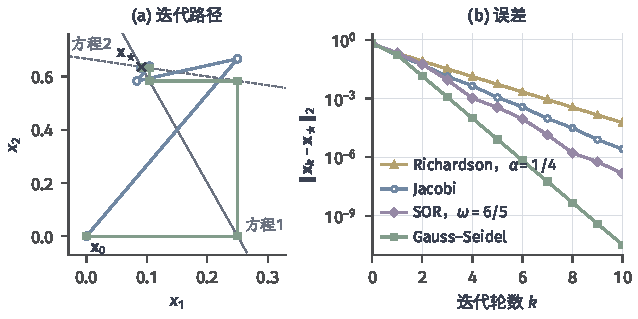
\includegraphics[width=108mm]{figures/01-basic-mathematics/03-vectors-matrices-and-multivariate-functions/matplotlib/c5-stationary-iteration-paths/figure.pdf}
  \caption{定常迭代在贯穿例$\bm A=\begin{bmatrix}4&1\\1&3\end{bmatrix}$，$\bm b=(1,2)^\top$，$\bm x_0=\bm 0$上的真实迭代值。左：实线与虚线分别是第一、第二个方程的解集，两者交于$\bm x_\star=(1/11,7/11)^\top$；蓝色圆点为Jacobi前四轮的迭代点，绿色折线为Gauss--Seidel前三轮的逐坐标路径。右：Richardson（$\alpha=1/4$）、Jacobi、SOR（$\omega=6/5$）与Gauss--Seidel的误差$\lVert\bm x_k-\bm x_\star\rVert_2$，纵轴取对数，渐近斜率分别对应谱半径约$0.40$、$0.29$、$0.20$与$1/12$。}
  \label{fig:ls-stationary-iteration-paths}
\end{figure}

\section{SOR迭代}
\label{sec:ls-sor}

\subsection{主要思想}

Gauss--Seidel每次坐标修正都恰好让当前方程成立，修正幅度是固定的。\term{逐次超松弛迭代}（successive over-relaxation，SOR）引入固定的\term{松弛参数}（relaxation parameter）$\omega\neq0$，调节每次坐标修正走多远。目的是在误差沿同一方向缓慢衰减时走得更快，或在修正过冲时收敛得更稳。

具体做法分两步。处理第$i$行时，先用当前可用的数据算出Gauss--Seidel候选值
\[
\widehat x_i=\frac{b_i-\sum_{j<i}a_{i,j}(\bm x_{k+1})_j-\sum_{j>i}a_{i,j}(\bm x_k)_j}{a_{i,i}} ,
\]
再让旧值朝候选值移动$\omega$倍的距离：
\[
(\bm x_{k+1})_i=(\bm x_k)_i+\omega\bigl(\widehat x_i-(\bm x_k)_i\bigr)=(1-\omega)(\bm x_k)_i+\omega\widehat x_i .
\]
$\omega=1$就是Gauss--Seidel；$0<\omega<1$称为欠松弛，只走一部分；$\omega>1$称为过松弛，越过候选值继续走。松弛参数改变的是修正，目标方程没有变。

松弛发生在每个坐标内部：后面的行读到的是前面已经松弛后的值。先做一次完整的Gauss--Seidel扫掠、再把整个向量与旧向量按$\omega$线性组合，一般得到的是另一种方法，不是逐坐标的SOR。

对应的分裂可以照Gauss--Seidel的办法得到。把分量式乘$a_{i,i}$并把本轮新量移到左边，合起来是
\[
(\bm D+\omega\bm L)\bm x_{k+1}=\omega\bm b+\bigl[(1-\omega)\bm D-\omega\bm U\bigr]\bm x_k .
\]
两边减去$(\bm D+\omega\bm L)\bm x_k$，右边化为$\omega(\bm b-\bm D\bm x_k-\bm L\bm x_k-\bm U\bm x_k)=\omega\bm r_k$，即
\[
(\bm D+\omega\bm L)\bm\delta_k=\omega\bm r_k ,\qquad
\bm M=\frac1\omega\bm D+\bm L .
\]
$\omega$同时影响每个坐标的修正幅度与整轮的误差传播，收敛条件在算法分析中讨论。

\subsection{算法实现}

\paragraph{松弛前代}
输入除初值、容差和上限外还有$\omega$，并记录变量顺序。参数是否合格与矩阵是否满足假设是两项不同的检查：对称正定情形的保证要求$0<\omega<2$，同时要求$\bm A$确实对称正定。每轮通过检查后，按既定顺序求解$(\bm D+\omega\bm L)\bm\delta_k=\omega\bm r_k$，即
\[
(\bm\delta_k)_i=\frac{\omega}{a_{i,i}}\Bigl((\bm r_k)_i-\sum_{j<i}a_{i,j}(\bm\delta_k)_j\Bigr),\qquad i=1,\ldots,d .
\]
计算当前分量时用到的，已经是前面分量松弛后的修正；$\omega=1$时这一步逐项退化为Gauss--Seidel的前代。

\paragraph{直接更新与检查}
等价地，可以原位逐坐标更新：对$i=1,\ldots,d$保存旧分量，算出$\widehat x_i$，写回$(1-\omega)(\bm x_k)_i+\omega\widehat x_i$；已访问的坐标立即供后面的行读取，未访问的坐标保持旧值。一轮结束后重算残差，满足容差才以成功返回。

\begin{example}[SOR迭代的前两轮]
\label{ex:ls-sor-first-sweep}
在例~\ref{ex:ls-stationary-running-example}中取$\omega=6/5$。第一轮中，第一行的候选值为$1/4$，松弛后$(\bm x_1)_1=\tfrac65\cdot\tfrac14=3/10$；第二行用这个松弛后的值，候选值为$(2-3/10)/3=17/30$，于是$(\bm x_1)_2=\tfrac65\cdot\tfrac{17}{30}=17/25$。所以$\bm x_1=(3/10,\,17/25)^\top$，残差$\bm r_1=(-22/25,\,-17/50)^\top$。

第二轮先算
\[
(\bm x_2)_1=-\tfrac15\cdot\tfrac3{10}+\tfrac65\cdot\frac{1-17/25}{4}=\frac9{250},
\]
再用它算
\[
(\bm x_2)_2=-\tfrac15\cdot\tfrac{17}{25}+\tfrac65\cdot\frac{2-9/250}{3}=\frac{406}{625},
\]
残差$\bm r_2=(129/625,\,19/1250)^\top$。

与例~\ref{ex:ls-gauss-seidel-first-sweep}不同，第二个方程不再恰好成立，因为它的修正被放大了五分之一。若先做完整一轮Gauss--Seidel、再按$\omega$把它与旧向量组合，得到的是$\tfrac65(1/4,7/12)^\top=(3/10,7/10)^\top$，与$\bm x_1$不同。

就这个例子而言，过松弛并没有带来好处：两轮的残差长度约为$0.94$与$0.21$，都大于Gauss--Seidel的$0.58$与$0.049$。有限轮的算例只用来解释计算过程；参数的优劣要由下面的谱半径判断。
\end{example}

\subsection{算法分析}

\paragraph{收敛条件}
SOR的迭代矩阵为
\[
\bm T_\omega=\bm I-\omega(\bm D+\omega\bm L)^{-1}\bm A=(\bm D+\omega\bm L)^{-1}\bigl[(1-\omega)\bm D-\omega\bm U\bigr].
\]
松弛参数不能随意取：它的取值范围对一般矩阵有一条必要条件，对实对称正定矩阵则恰好也是充分条件。
\begin{theorem}[SOR迭代的收敛条件]
\label{thm:ls-sor-convergence}
设$\bm A$的对角元全不为零。
\begin{enumerate}
\item 对任意这样的方阵，$\rho(\bm T_\omega)\geq|1-\omega|$；所以SOR对所有初值收敛的必要条件是$0<\omega<2$。
\item 若$\bm A$实对称正定且$0<\omega<2$，则$\rho(\bm T_\omega)<1$，SOR对所有初值收敛。
\end{enumerate}
\end{theorem}
\begin{proof}
（1）$\bm D+\omega\bm L$是下三角阵，行列式为$\prod_i a_{i,i}$；$(1-\omega)\bm D-\omega\bm U$是上三角阵，行列式为$(1-\omega)^d\prod_i a_{i,i}$。所以$\det\bm T_\omega=(1-\omega)^d$。行列式等于全部特征值之积，其模不超过$\rho(\bm T_\omega)^d$，故$\rho(\bm T_\omega)\geq|1-\omega|$。若$\omega\leq0$或$\omega\geq2$，则$\rho(\bm T_\omega)\geq1$，由定理~\ref{thm:ls-stationary-convergence}不能对所有初值收敛。

（2）第$i$次坐标修正的步长是$t=\omega r_i/a_{i,i}$，代入定理~\ref{thm:ls-gauss-seidel-convergence}证明中的能量变化式，$\phi$减少
\[
\omega\frac{r_i^2}{a_{i,i}}-\frac{\omega^2}{2}\frac{r_i^2}{a_{i,i}}=\frac{\omega(2-\omega)\,r_i^2}{2a_{i,i}} .
\]
当$0<\omega<2$时这是非负量，且只在$r_i=0$时为零。此后的论证与该证明相同：一整轮能量不减少只能是$\bm e_k=\bm0$，于是$\bm A-\bm T_\omega^\top\bm A\bm T_\omega$正定，再由特征向量的二次型得$\rho(\bm T_\omega)<1$。
\end{proof}

\paragraph{参数选择与代价}
区间内收敛不等于每个参数都比Gauss--Seidel快。收敛速度取决于参数和变量排列：三对角等特殊结构的矩阵有由$\rho(\bm T_{\mathrm J})$给出的最优参数公式，但不能普遍套用。贯穿例的$\omega=6/5$就使谱半径从Gauss--Seidel的$1/12$升到$0.2$。$\omega$接近区间端点时，由第一部分$\rho(\bm T_\omega)\geq|1-\omega|$接近一，收敛可能很弱。一轮成本与Gauss--Seidel同阶。

\section{SSOR迭代}
\label{sec:ls-ssor}

\subsection{主要思想}

单向扫掠依赖变量顺序，对应的$\bm M=\bm D/\omega+\bm L$也不对称。对实对称正定的$\bm A$，\term{对称逐次超松弛迭代}（symmetric SOR，SSOR）把一次前向SOR扫掠与一次反向SOR扫掠配成一轮，超参数取固定的$0<\omega<2$。下面把两次修正合并成一个修正矩阵，并推导缩放常数，使独立迭代与作为预条件的实现使用同一约定。

对称性给出$\bm U=\bm L^\top$。记
\[
\bm F=\bm D+\omega\bm L,\qquad \bm F^\top=\bm D+\omega\bm U .
\]
前向半步就是一次SOR：解$\bm F\bm\delta_{\mathrm f}=\omega\bm r_k$，令$\bm x_{k+1/2}=\bm x_k+\bm\delta_{\mathrm f}$。反向半步按$i=d,\ldots,1$的顺序做SOR，此时先访问的是下标大的分量，所以新值出现在上三角部分，对应的方程是$\bm F^\top\bm\delta_{\mathrm b}=\omega\bm r_{k+1/2}$，再令$\bm x_{k+1}=\bm x_{k+1/2}+\bm\delta_{\mathrm b}$。右端必须是半步后的残差
\[
\bm r_{k+1/2}=\bm b-\bm A\bm x_{k+1/2}=\bm r_k-\bm A\bm\delta_{\mathrm f},
\]
第二次扫掠不能继续使用未经修正的旧残差。

把两次修正相加。由$\bm\delta_{\mathrm f}=\omega\bm F^{-1}\bm r_k$，
\[
\begin{aligned}
\bm\delta_{\mathrm f}+\bm\delta_{\mathrm b}
&=\omega\bm F^{-1}\bm r_k+\omega\bm F^{-\top}\bigl(\bm r_k-\omega\bm A\bm F^{-1}\bm r_k\bigr)\\
&=\omega\bm F^{-\top}\bigl(\bm F^\top\bm F^{-1}+\bm F\bm F^{-1}-\omega\bm A\bm F^{-1}\bigr)\bm r_k
=\omega\bm F^{-\top}\bigl(\bm F^\top+\bm F-\omega\bm A\bigr)\bm F^{-1}\bm r_k ,
\end{aligned}
\]
第二个等号在第一项前插入$\bm F^{-\top}\bm F^\top$，在第二项中插入$\bm F\bm F^{-1}$。又$\bm F^\top+\bm F-\omega\bm A=2\bm D+\omega(\bm L+\bm U)-\omega(\bm D+\bm L+\bm U)=(2-\omega)\bm D$，所以一整轮的修正为
\[
\bm\delta_k=\omega(2-\omega)\,\bm F^{-\top}\bm D\bm F^{-1}\bm r_k .
\]

于是SSOR的一轮等价于以
\[
\bm M_{\mathrm{SSOR}}=\frac{1}{\omega(2-\omega)}(\bm D+\omega\bm L)\bm D^{-1}(\bm D+\omega\bm U)
=\frac{1}{\omega(2-\omega)}\bm F\bm D^{-1}\bm F^\top
\]
为修正矩阵的定常迭代：$\bm M_{\mathrm{SSOR}}\bm\delta_k=\bm r_k$。求解的次序是先解$\bm F$、再乘$\bm D$、最后解$\bm F^\top$，不必显式形成$\bm M_{\mathrm{SSOR}}$或它的逆。

这个修正矩阵对称正定。对称性由形式$\bm F\bm D^{-1}\bm F^\top$直接看出。$\bm A$正定使对角元$a_{i,i}=\bm e_i^\top\bm A\bm e_i>0$，所以$\bm D\succ0$；$\bm F$是对角元为正的下三角阵，可逆。于是对$\bm v\neq\bm0$，
\[
\bm v^\top\bm M_{\mathrm{SSOR}}\bm v=\frac{(\bm F^\top\bm v)^\top\bm D^{-1}(\bm F^\top\bm v)}{\omega(2-\omega)}>0 ,
\]
这里用到$0<\omega<2$使分母为正。注意对称正定的是修正矩阵$\bm M_{\mathrm{SSOR}}$；迭代矩阵$\bm I-\bm M_{\mathrm{SSOR}}^{-1}\bm A$一般不是对称矩阵。正是$\bm M_{\mathrm{SSOR}}$的对称正定性，使SSOR除了单独迭代，还能为第~\ref{chap:krylov-methods}章的共轭梯度法提供预条件。

\subsection{算法实现}

\paragraph{双向扫掠}
内部状态除$\bm x_k,\bm r_k$外，多一个半步向量$\bm x_{k+1/2}$。第一步按SOR的分量公式完成$i=1,\ldots,d$的前向扫掠，得到$\bm x_{k+1/2}$。第二步反向遍历$i=d,\ldots,1$：
\[
(\bm x_{k+1})_i=(1-\omega)(\bm x_{k+1/2})_i+\frac{\omega}{a_{i,i}}\Bigl(b_i-\sum_{j<i}a_{i,j}(\bm x_{k+1/2})_j-\sum_{j>i}a_{i,j}(\bm x_{k+1})_j\Bigr),
\]
下标比$i$大的分量已在本次反向扫掠中更新，比$i$小的仍是半步值。原位覆盖同样成立。

\paragraph{因子求解}
等价的实现直接按$\bm M_{\mathrm{SSOR}}$的三个因子求修正量。从$\bm r_k=\bm b-\bm A\bm x_k$出发，依次
\[
\bm F\bm y=\bm r_k,\qquad \bm t=\bm D\bm y,\qquad \bm F^\top\bm z=\bm t,\qquad \bm\delta_k=\omega(2-\omega)\bm z ,
\]
其中第一步是第~\ref{sec:ls-lu}节的前代，第三步是回代；最后令$\bm x_{k+1}=\bm x_k+\bm\delta_k$，重算$\bm r_{k+1}=\bm b-\bm A\bm x_{k+1}$并检查终止。由主要思想中的推导，这四步与双向扫掠的缩放完全对应。

\begin{example}[SSOR迭代的前两轮]
\label{ex:ls-ssor-two-sweeps}
在例~\ref{ex:ls-stationary-running-example}中取$\omega=1$。按双向扫掠，前向半步就是一轮Gauss--Seidel，$\bm x_{1/2}=(1/4,\,7/12)^\top$。反向扫掠先处理第二行，$(\bm x_1)_2=(2-1/4)/3=7/12$，保持不变；再处理第一行，用刚得到的第二分量，$(\bm x_1)_1=(1-7/12)/4=5/48$。

按因子路径核对同一轮：$\bm F=\left[\begin{smallmatrix}4&0\\1&3\end{smallmatrix}\right]$，解$\bm F\bm y=\bm b$得$\bm y=(1/4,7/12)^\top$；$\bm t=\bm D\bm y=(1,7/4)^\top$；解$\bm F^\top\bm z=\bm t$，先得$z_2=7/12$，再得$z_1=(1-7/12)/4=5/48$。此时$\omega(2-\omega)=1$，$\bm x_1=\bm z=(5/48,\,7/12)^\top$，与双向扫掠一致。

用原方程重算，第一轮的真实残差为$\bm r_1=(0,\,7/48)^\top$。这次为零的是第一个分量，因为反向扫掠最后修正的是第一行。第二轮得到
\[
 \bm x_2=(53/576,\,91/144)^\top,\qquad \bm r_2=(0,\,7/576)^\top .
\]
两轮中各个三角子问题都精确解出了，残差却仍不为零。验收用的是原方程的残差，不能以子问题已经解完代替。
\end{example}

\paragraph{作为预条件}
作为共轭梯度法的预条件使用时，SSOR不更新近似解，只把外层迭代给出的残差$\bm r$变成修正方向：执行$\bm F\bm y=\bm r$、$\bm t=\bm D\bm y$、$\bm F^\top\bm z=\bm t$及缩放，返回$\bm M_{\mathrm{SSOR}}^{-1}\bm r$，近似解由外层方法另行更新。同一次外层求解中，$\omega$和三角因子要保持不变，否则预条件矩阵逐轮变化，外层方法依赖的固定内积结构就不成立。具体用法见第~\ref{sec:ls-preconditioning}节。

\subsection{算法分析}

\paragraph{收敛性}
$\bm M_{\mathrm{SSOR}}$正定本身还不足以断言定常迭代收敛；还需要它在二次型意义下不小于$\bm A$。展开$\bm F\bm D^{-1}\bm F^\top=\bm D+\omega\bm L+\omega\bm U+\omega^2\bm L\bm D^{-1}\bm U$，减去$\omega(2-\omega)\bm A=\omega(2-\omega)(\bm D+\bm L+\bm U)$，整理得
\[
\omega(2-\omega)(\bm M_{\mathrm{SSOR}}-\bm A)
=(1-\omega)^2\bm D-\omega(1-\omega)(\bm L+\bm U)+\omega^2\bm L\bm D^{-1}\bm U
=\bm C\bm D^{-1}\bm C^\top ,
\]
其中$\bm C=(1-\omega)\bm D-\omega\bm L$，最后一步把$\bm C\bm D^{-1}\bm C^\top$展开即可核对。因为$\bm D\succ0$，$\bm C\bm D^{-1}\bm C^\top\succeq0$，所以
\[
\bm 0\prec\bm A\preceq\bm M_{\mathrm{SSOR}} .
\]

由此读出迭代矩阵的谱。$\bm M_{\mathrm{SSOR}}$对称正定，有正定平方根（第~\ref{sec:ls-matrix-square-root}节）。令$\bm S=\bm M_{\mathrm{SSOR}}^{-1/2}\bm A\bm M_{\mathrm{SSOR}}^{-1/2}$，它实对称。若$\bm S\bm w=\mu\bm w$，$\bm w\neq\bm0$，令$\bm y=\bm M_{\mathrm{SSOR}}^{-1/2}\bm w$，则
\[
\mu=\frac{\bm w^\top\bm S\bm w}{\bm w^\top\bm w}=\frac{\bm y^\top\bm A\bm y}{\bm y^\top\bm M_{\mathrm{SSOR}}\bm y}\in(0,1].
\]
迭代矩阵$\bm T_{\mathrm{SSOR}}=\bm I-\bm M_{\mathrm{SSOR}}^{-1}\bm A=\bm M_{\mathrm{SSOR}}^{-1/2}(\bm I-\bm S)\bm M_{\mathrm{SSOR}}^{1/2}$与实对称矩阵$\bm I-\bm S$相似，特征值$1-\mu$全部落在$[0,1)$中，所以$\rho(\bm T_{\mathrm{SSOR}})<1$。由定理~\ref{thm:ls-stationary-convergence}，在$\bm A$实对称正定、$0<\omega<2$时SSOR对所有初值收敛。这里$\bm T_{\mathrm{SSOR}}$本身一般不对称，只是相似于对称矩阵，因而特征值为实数。

\paragraph{代价与用途}
一轮含两次三角扫掠（或等价的前代、对角缩放与回代），另加一次计算残差的矩阵乘向量，工作量约为SOR一轮的两倍；存储只多一个与$\bm x$同长的中间向量。比较时不能只数轮数：贯穿例中$\omega=1$的SSOR谱半径为$1/12$，与Gauss--Seidel相同，每轮却多花一倍计算。SSOR作为独立迭代往往并不比SOR省；它的主要价值在于对称正定的修正矩阵：作为预条件时，每次外层迭代多付两次三角求解，换来外层共轭梯度法所需步数的减少，是否划算要按总成本比较（第~\ref{sec:ls-preconditioning}节）。

\section{收敛检验与停止准则}
\label{sec:ls-stationary-stopping}

各方法都使用第~\ref{sec:ls-matrix-splitting}节的终止条件：$\lVert\bm r_k\rVert_2\leq\mathrm{atol}+\mathrm{rtol}\lVert\bm b\rVert_2$，或$k=K$。前者表示达到了给定的残差要求；后者只表示不再继续计算，结果未必达到精度。两种情况下输出都只是当前的$\bm x_k$，所以结束状态必须一并报告。残差用真实的$\bm b-\bm A\bm x_k$计算，而不是只依赖递推值。

几种量不能代替原方程的残差检验。修正量$\lVert\bm\delta_k\rVert$很小，可能只说明收缩因子接近一、迭代走得很慢，而不是已经接近解。残差在很多轮内几乎不降，应作为停滞报告，而不是当作收敛。计算中出现溢出或非数，应作为数值异常报告；这通常说明迭代发散或对角元过小。

残差小也不等于解的误差小。由$\bm x_\star-\bm x_k=\bm A^{-1}\bm r_k$，误差是残差经$\bm A^{-1}$放大的结果，两者之间隔着问题本身的敏感性；第~\ref{sec:ls-numerical-sensitivity}节再给出误差界和后向误差的解释。比较不同方法时，应在相同精度要求下比较总工作量，而不是轮数；分析中的收敛率和代价用于解释算法，不加入求解器的输出。其他用递推方式维护残差的方法，递推值会因舍入而偏离真实残差，停止前也须用$\bm b-\bm A\bm x_k$复核。

\FloatBarrier
\section{本章小结}
\label{sec:stationary-iterations-summary}

本章回答了怎样不分解$\bm A$而逐步求解可逆方程$\bm A\bm x=\bm b$。共同的做法是矩阵分裂$\bm A=\bm M-\bm N$：每轮解一个以易解矩阵$\bm M$为系数的修正方程$\bm M\bm\delta_k=\bm r_k$，再更新近似解。误差满足$\bm e_{k+1}=(\bm I-\bm M^{-1}\bm A)\bm e_k$，由第~\ref{chap:linear-recurrence-stability}章的矩阵幂结论，迭代对任意初值收敛当且仅当迭代矩阵的谱半径小于一，渐近速度也由谱半径决定。

五种方法的区别只在于$\bm M$怎样近似$\bm A$、数据怎样读取。Richardson取$\bm M=\alpha^{-1}\bm I$，只需矩阵乘向量；对称正定时收敛当且仅当$0<\alpha<2/\lambda_{\max}$，最优步长的收缩因子为$(\kappa_2-1)/(\kappa_2+1)$。Jacobi取$\bm M=\bm D$，各分量只读旧值、可以并行，严格行对角占优保证收敛，对称正定本身不保证。

Gauss--Seidel取$\bm M=\bm D+\bm L$，立即使用本轮新值，相当于一次前代；严格行对角占优或对称正定都保证收敛。SOR取$\bm M=\bm D/\omega+\bm L$，$0<\omega<2$对一般矩阵是必要条件，对对称正定矩阵也是充分条件；区间内不同参数的速度仍须比较。SSOR把前向与反向SOR配成一轮，修正矩阵$\bm M_{\mathrm{SSOR}}=\bm F\bm D^{-1}\bm F^\top/[\omega(2-\omega)]$对称正定且满足$\bm A\preceq\bm M_{\mathrm{SSOR}}$，由此证明收敛，并可作为共轭梯度法的预条件。

这些结论都有边界。对角元非零只保证可执行，不保证收敛；用了新信息、加了过松弛，都不自动更快；贯穿例中Gauss--Seidel的谱半径为$1/12$，$\omega=6/5$的SOR反而是$0.2$。比较方法要把谱半径决定的轮数与每轮成本合起来，看达到相同精度的总工作量。

停止计算也要分清含义。只有真实残差满足$\lVert\bm r_k\rVert_2\leq\mathrm{atol}+\mathrm{rtol}\lVert\bm b\rVert_2$才算达到残差目标；步数耗尽、停滞或数值异常都只是停止，修正量很小也不代表接近解。即使残差达标，前向误差仍受问题条件数制约，这在第~\ref{sec:ls-numerical-sensitivity}节讨论；第~\ref{chap:krylov-methods}章则在逐步扩大的子空间中选择近似，以改善定常迭代受谱半径限制的收敛速度。
